\documentclass[12pt]{report}
\usepackage{uhthesis3}
\usepackage{booktabs}
\usepackage[small,bf]{caption}
\usepackage{graphicx}
\usepackage{subfig}
\usepackage{lscape}
\usepackage{algorithm}
\usepackage{algorithmic}
\usepackage{listings}
% \usepackage{courier}
\usepackage[titletoc]{appendix}

% LAD definitions
\def\vx{{\vec x}}
\def\vxdot{{\dot\vx}} \def\vxddot{{\ddot\vx}}
\def\tpose{^\top}
\def\ru{{\rm u}}
\def\vc{{\vec c}}
\def\vrho{{{\bf p}}}
\def\mat#1{{\bf#1}}
\def\vec#1{{\bf#1}}
\def\bold#1{\setbox0=\hbox{#1}
 \kern-.025em\copy0\kern-\wd0
 \kern.05em\copy0\kern-\wd0
 \kern-.025em\raise.0433em\box0}
\def\vsigma{{\bf \sigma}}
\def\vepsilon{{\bf \epsilon}}
\def\ssqueeze{\vspace{-0.5cm}}

\def\bsqueeze{\vspace*{-0.8cm}}
\def\bpsqueeze{\vspace*{-0.6cm}}
\def\asqueeze{\vspace{-0.5cm}}


\def\inv{^{-1}}
\def\vuhat{{\hat \vec u}}
\def\avtk{{t_{k}}}
\def\bvtk{{t_{k+1}}}
\def\vu{{\vec u}}
\def\vuhat{{\hat \vec u}}
\def\vq{{\vec q}}
\def\vqdot{{\dot\vq}}
\def\tpose{^\top}
\def\mat#1{{\bf#1}}
\def\extvec#1#2#3{{~^{#1}{\bf#2}_{#3}}}
\def\extvecrm#1#2#3{{~^{{\rm #1}}{\bf#2}_{#3}}}

\def\cavindex{{\cal V\cal I}}
\def\caawpoint{{\extvec{\Phi}{x}{j}}}
\def\caaipointrm{{\extvecrm{I}{x}{j}}}
\def\caaipoint{{\extvec{I}{x}{j}}}

\newcounter{lfigcounter}
\newenvironment{IonTab}{\begin{table}[htb]}{\end{table}}
\newenvironment{IonFig}{\setcounter{lfigcounter}{1}\begin{figure}}{\end{figure}}
\newenvironment{IonFigH}{\setcounter{lfigcounter}{1}\begin{figure}[h]}{\end{figure}}
\newenvironment{IonFigT}{\setcounter{lfigcounter}{1}\begin{figure}[t]}{\end{figure}}
\def\ionbox#1{\makebox[#1]{(\alph{lfigcounter})}\stepcounter{lfigcounter}}

%%%%%%%%%%%%%%%%%%%%%%%%%%%%%%%%%%%%%%%%%%%%%%%%%%%%%%%%%%%%%%5

\setcounter{secnumdepth}{4}

\begin{document}

\title{\bf \large Mavis: Visualization Tool for Multiple Sequence Alignments}
\author{Lei Zhao}
\submitdate{May 2011} \degree{Master of Science}{Thesis}
\adviser{Dr. Yuriy Fofanov, Chairman\\
Department of Computer Science }
\firstreader{Dr. Dan Graur \\
Department of Biology and Biochemistry}
\secondreader{Dr. Shishir Shah\\
Department of Computer Science}
\threereadersfalse
\fourreadersfalse
\fivereadersfalse

\copyrightfalse \makecoverpages
\begin{acknowledgements}
I am very grateful to my thesis supervisors, Dr. Dan Graur and Dr. Reed A. Cartwright, for their guidance, encouragement, patience, and support during the course of this work. I have encountered may difficulties, but your help made this thesis possible.

I would like to thank Dr. Yuriy Fofanov and Dr. Shishir Shah for being my thesis committee members and providing valuable suggestions.

I would like to thank my lab mates, Dr. Giddy Landan, Dr. Kiyoshi Izawa, Dr. Niv Sabath, Nicholas Price, Longyi Qi, and Yichen Zheng. I had a great time in this lab for two years and learned a lot.

I would like to thank my other friends in the University of Houston for all their support, entertainment, and caring.

My special thank goes to my wife Bingjun Zhang, my parents Dr. Wenyuan Zhao and Yijun Wang, and my previous supervisor when I was in China, Dr. Kui Lin. They are the most important persons in my life. To them I dedicate this thesis.

\end{acknowledgements}

\begin{abstract}
\emph{(Under construction)}

\end{abstract}
\setlength{\parskip}{.1 in}

\makecontentspages

\chapterpages
\newif \ifFIGS
\FIGSfalse

\chapter{Introduction}\label{chap:Introduction}

\section{Background}

Multiple sequence alignment (MSA) analysis, a fundamental approach in molecular biology, is required for nearly all comparative sequence studies, including evolutionary, functional and structural aspects. A multiple sequence alignment is usually a matrix, in which each row represents a sequence, and each column corresponds to the equivalent positions across all sequences aligned. Each element of the matrix contains a symbol, which can be either `-' (a gap) or a sequence symbol (an amino acid for DNA/RNA sequences, or a nucleotide base for protein sequences). \cite{Edgar:2006aa}

Due to the size and complexity of the multiple sequence alignment datasets, computer visualization techniques are essential to assist in understanding, analyzing and evaluating the alignment results. Numerous MSA visualization applications, either stand-alone or web-based, have been developed in recent decades, ranging from simple MSA viewers, to complex editing and analysis platforms. Many of them have graphical user interfaces showing a grid of symbols, usually along with various coloring, sizing and annotation. \cite{Procter2010aa}

\section{Related Work}

Coloring an alignment has been widely implemented to highlight specific regions, properties or patterns. \cite{Procter2010aa} The simplest way of coloring is to use a fixed color scheme, in which each sequence symbol has its own color, and will not be changed across the alignment. The assignment of color schemes are usually based on some empirical properties or chemical classifications. There are numerous color schemes available for different purposes, but Taylor \cite{LIN2002361} and Clustal \cite{Thompsonaa} are widely used and often considered de facto standards.

However, using pre-determined color schemes to color sequence symbols, either amino acids or nucleotide bases, are not always helpful to phylogenetic analysis. Those fixed schemes focus on chemical differences between specific types of symbols, rather than between sequences, regions, blocks or structures of the alignment. For example, if symbols are examined within a certain column, the colors reflect the similarities fairly well. However, if the alignment is analyzed horizontally, comparative information within a row or a rectangular region are unable to be displayed, like how one sequence is similar with others, which section aligns better than another, which subset of sequences in which range of columns are more conserved, or how robust is the alignment accuracy.

Here we suggest a new MSA visualization tool, Mavis (Multiple Alignment VISualization), which focuses on highlighting evolutionary relationships and internal structures of an alignment. Instead of relying on chemical properties or any other information from symbol types, our approach takes only symbol-symbol correlation into consideration. The most valuable result we would like to provide is a whole picture of the MSA.

\section{Thesis Outline}

This thesis is organized in the following way: Chapter 2 briefly summarizes how Mavis processes data input, creates colors and displays the colored MSA graph. Chapter 3 explains the algorithm step by step, from scaling to mapping and optimization. Chapter 4 describes our implementation of the algorithm, including the back-end, API and front-end. Chapter 5 presents test results to show the validity and performance of our implementation. The whole work is discussed and concluded in Chapter 6.
\chapter{Approach}\label{chap:Approach}

\section{Main Objective}

In this thesis, we address a novel method to visualize multiple sequence alignments using colors. The main objective is to highlight sequence similarity (or alignment confidence) with color similarity.

In the alignment matrix, a well-aligned area should be represented by a solid-color shape, while a poorly-aligned one should become a mosaic of different colors. All the alignment-level information, such as evolutionary relationships, phylogenetic characteristics and alignment accuracy, should be revealed by the color pattern of the graph. Figure \ref{fig:app-wa} compares two types of MSA regions and their coloring results.

\begin{figure}[hbt]
\centering
\subfloat[A well-aligned MSA region.]{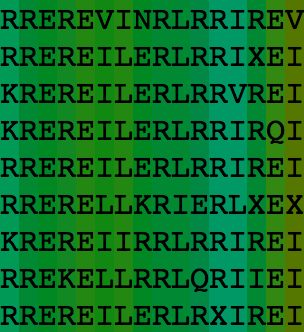
\includegraphics[width=0.35\textwidth]{figures/app-wa.png}}
\hspace{5mm}
\subfloat[A poorly-aligned MSA region.]{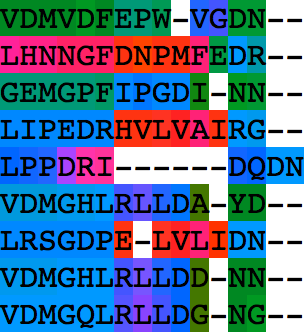
\includegraphics[width=0.35\textwidth]{figures/app-pa.png}}
\caption[Highlighting Sequence Similarity With Color Similarity]{Highlighting sequence similarity with color similarity.}\label{fig:app-wa}
\end{figure}

\section{Data Input}

Figure \ref{fig:app-wa}(a) shows a well-aligned MSA region, which contains many different types of amino acids. In order to demonstrate the good alignment quality, however, these amino acids need to be painted with similar colors. Obviously, the color assignment could not depend only on their types.

Unlike most traditional coloring approaches, we use an set of pairwise scores instead. Within each column of an MSA, all sequence residues are considered to be aligned together at the same equivalent position. We employ a third-party tool to examine each pair of these residues, and estimate the confidence that they should be aligned together. This confidence estimation can also be interpreted as a similarity score between the two residues.

Every pair of residues within a same column has a similarity score. These scores are used to determine how similar the residue colors should appear to each other. In a good-quality MSA region, all residues are confidently aligned together, therefore the colors would be almost the same. While in a bad-quality region, many alignments are doubtable, resulting in many different colors.

One good way to generate this similarity score data set is by using GUIDANCE \cite{Penn:2010aa,Penn:2010ab}, which is a tool for quantifying alignment uncertainty. GUIDANCE produces a confidence score in range of $[0, 1]$, named GUIDANCE score, for each symbol, symbol pair, column and sequence in the alignment. We take the symbol-pair GUIDANCE confidence scores as the input to Mavis.

\section{Color Generating}

The colors of the symbols are generated in such way that the color similarity represents the residue's alignment confidence. We have four steps to accomplish this goal.

\begin{figure}[hbt]
\center{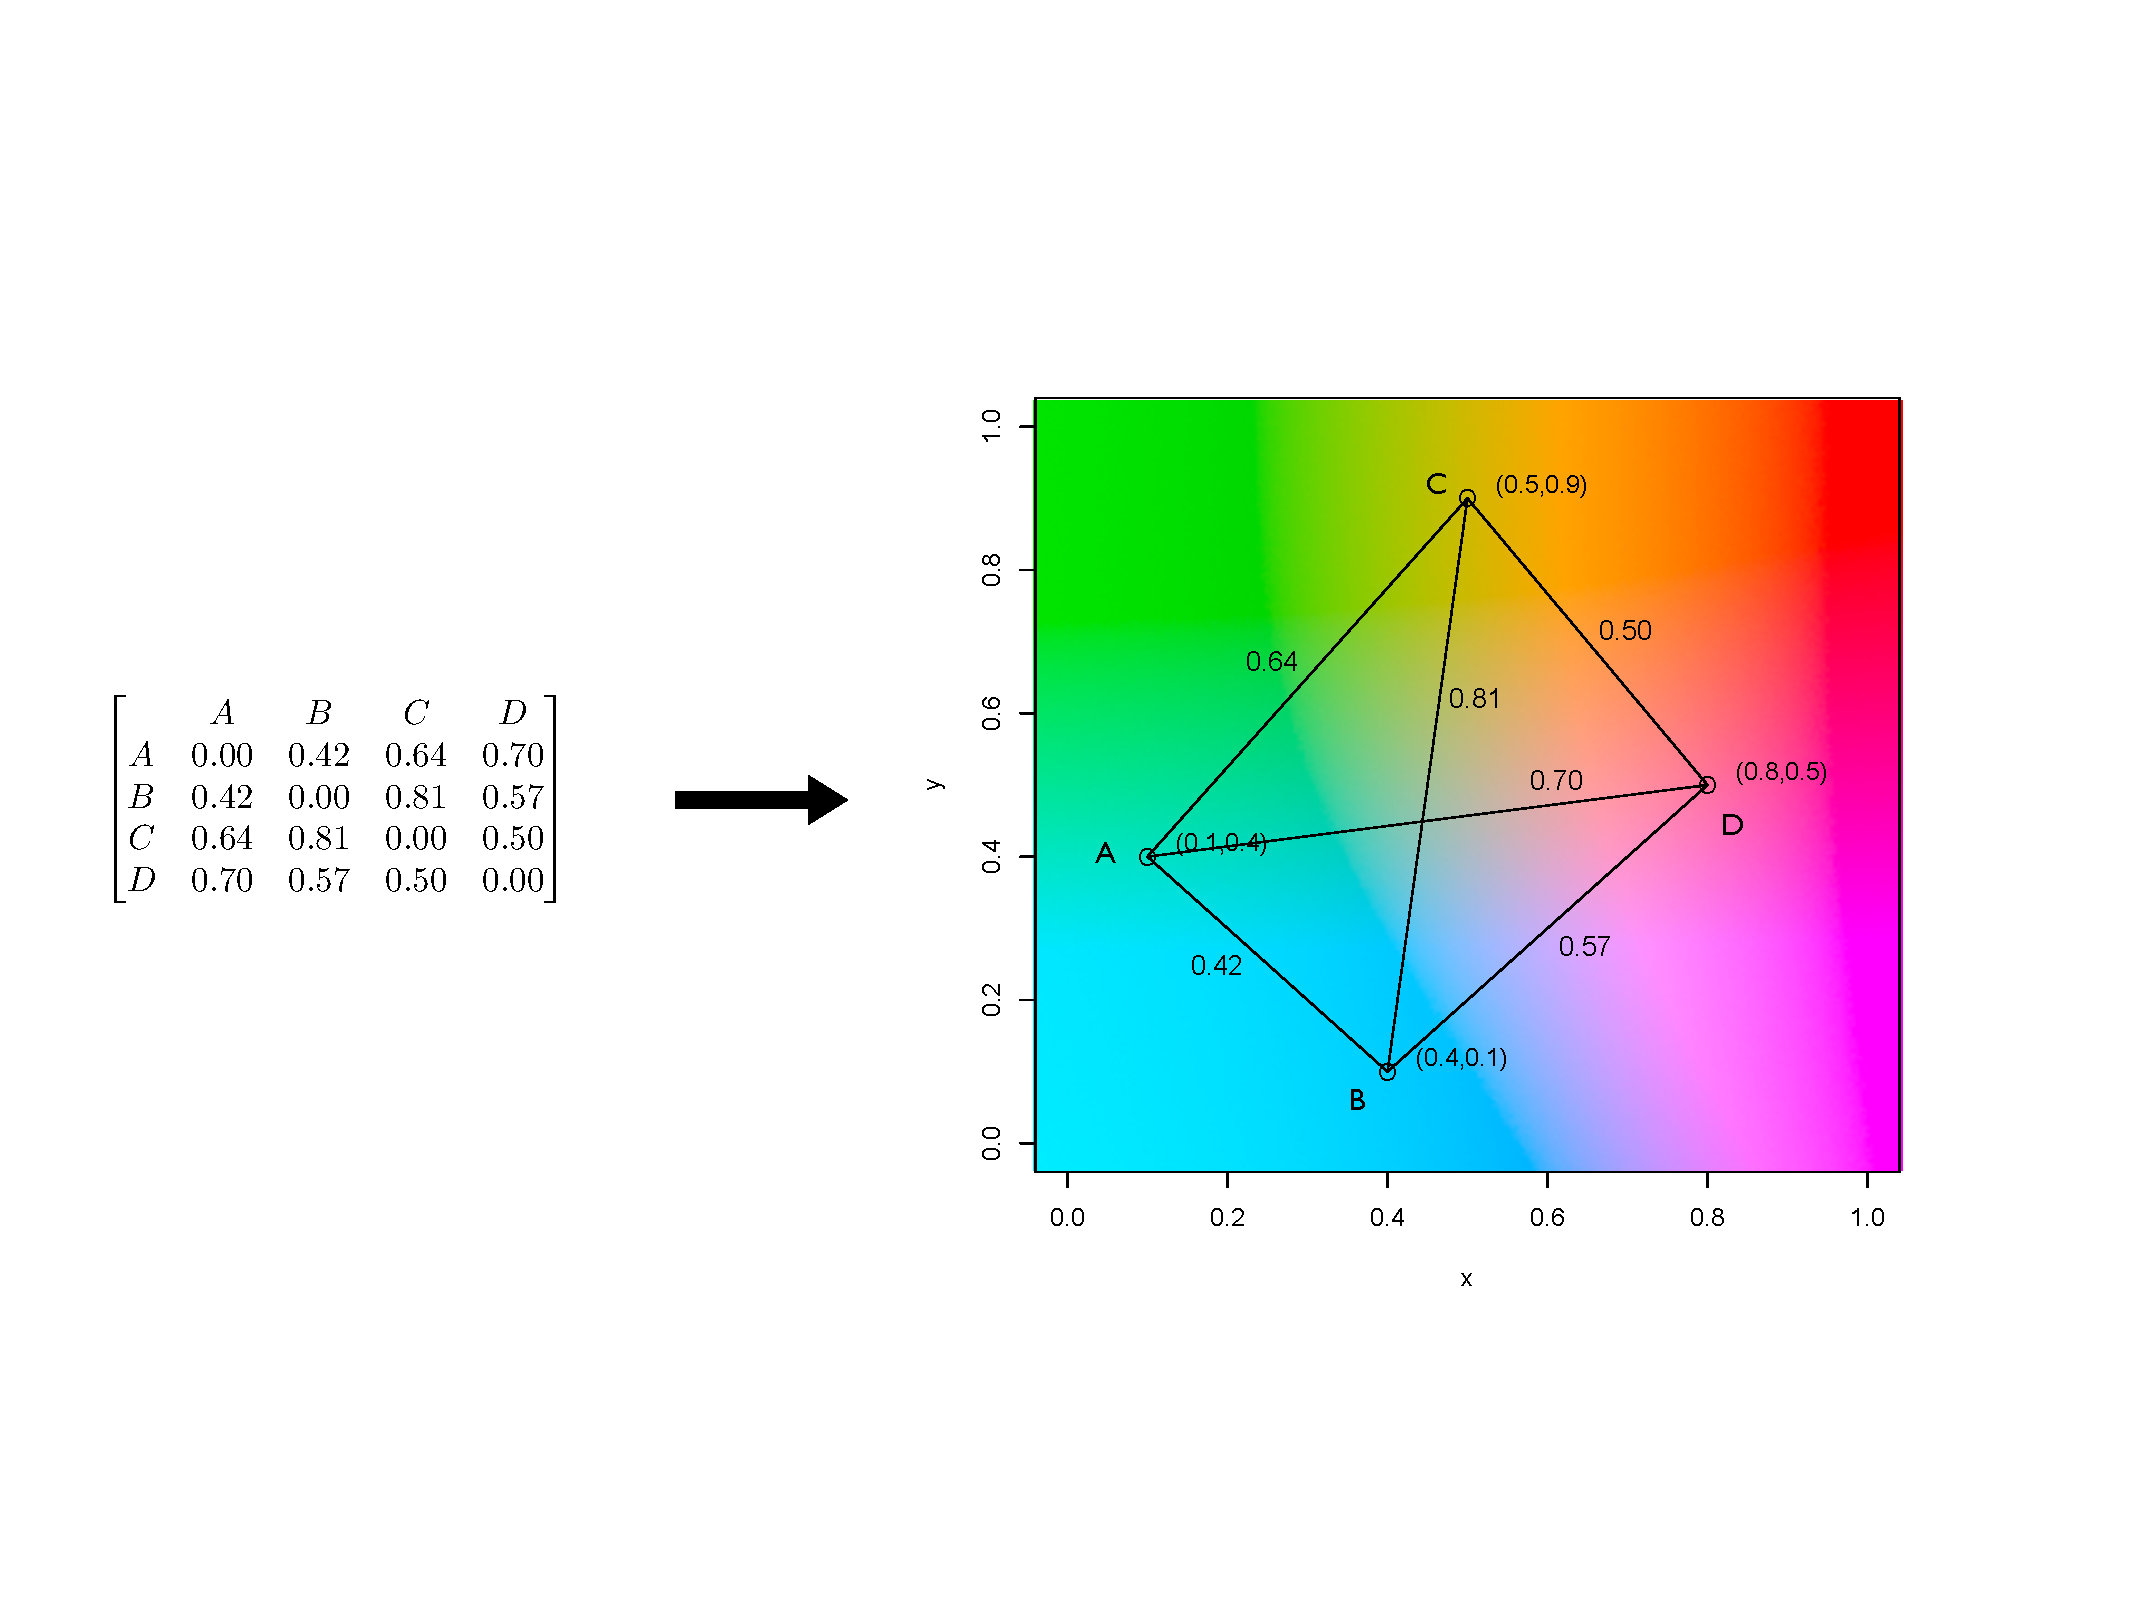
\includegraphics[width=\textwidth]{figures/chap2_color.pdf}}
\caption[Conversion from Distance Matrix into Colors]{A distance matrix is converted into points on a two-dimensional color space. The distances between points are approximately preserved. The color where a point is located is assigned to the corresponding alignment residue.}\label{fig:chap2_color}
\end{figure}

First, the confidence or similarity score is converted into a distance or dissimilarity score. Second, from all these distances, an $N*N$ distance matrix is constructed for each column, where $N$ is the number of residues in the same column. Third, from the distance matrix, the $N$ residues are mapped as $N$ points in a space of $N-1$ dimensions, such that for each pair of points, their Euclidean distance is equal to the value in the distance matrix. Finally, we map this space onto a color space, to find a color for each point. In an appropriate color space, the Euclidean distance approximately represents the color difference perceived by humans, so that our alignment confidence is linked with color similarity.

One problem is, most color spaces are three-dimensional or under. In order to map the original space to a color space, it is necessary to reduce the dimension from $N-1$ to no more than 3, while the distances are still preserved as much as possible. This dimension reduction process is done by using a statistical technique called \emph{classical multidimensional scaling} \cite{Borg:1997aa}.

\section{Color Optimization}

Up to now, our approach only operates on the column level, and does not consider the relationship between columns. The only way to create a solid-color well-aligned region, is to take cross-column information into account. Since there is no confidence score for two residues from different columns, the color difference between them does not mean anything, and should be eliminated as much as we can. In other words, the color graph needs to be as smooth as possible in the horizontal direction.

\begin{figure}[hbt]
\center{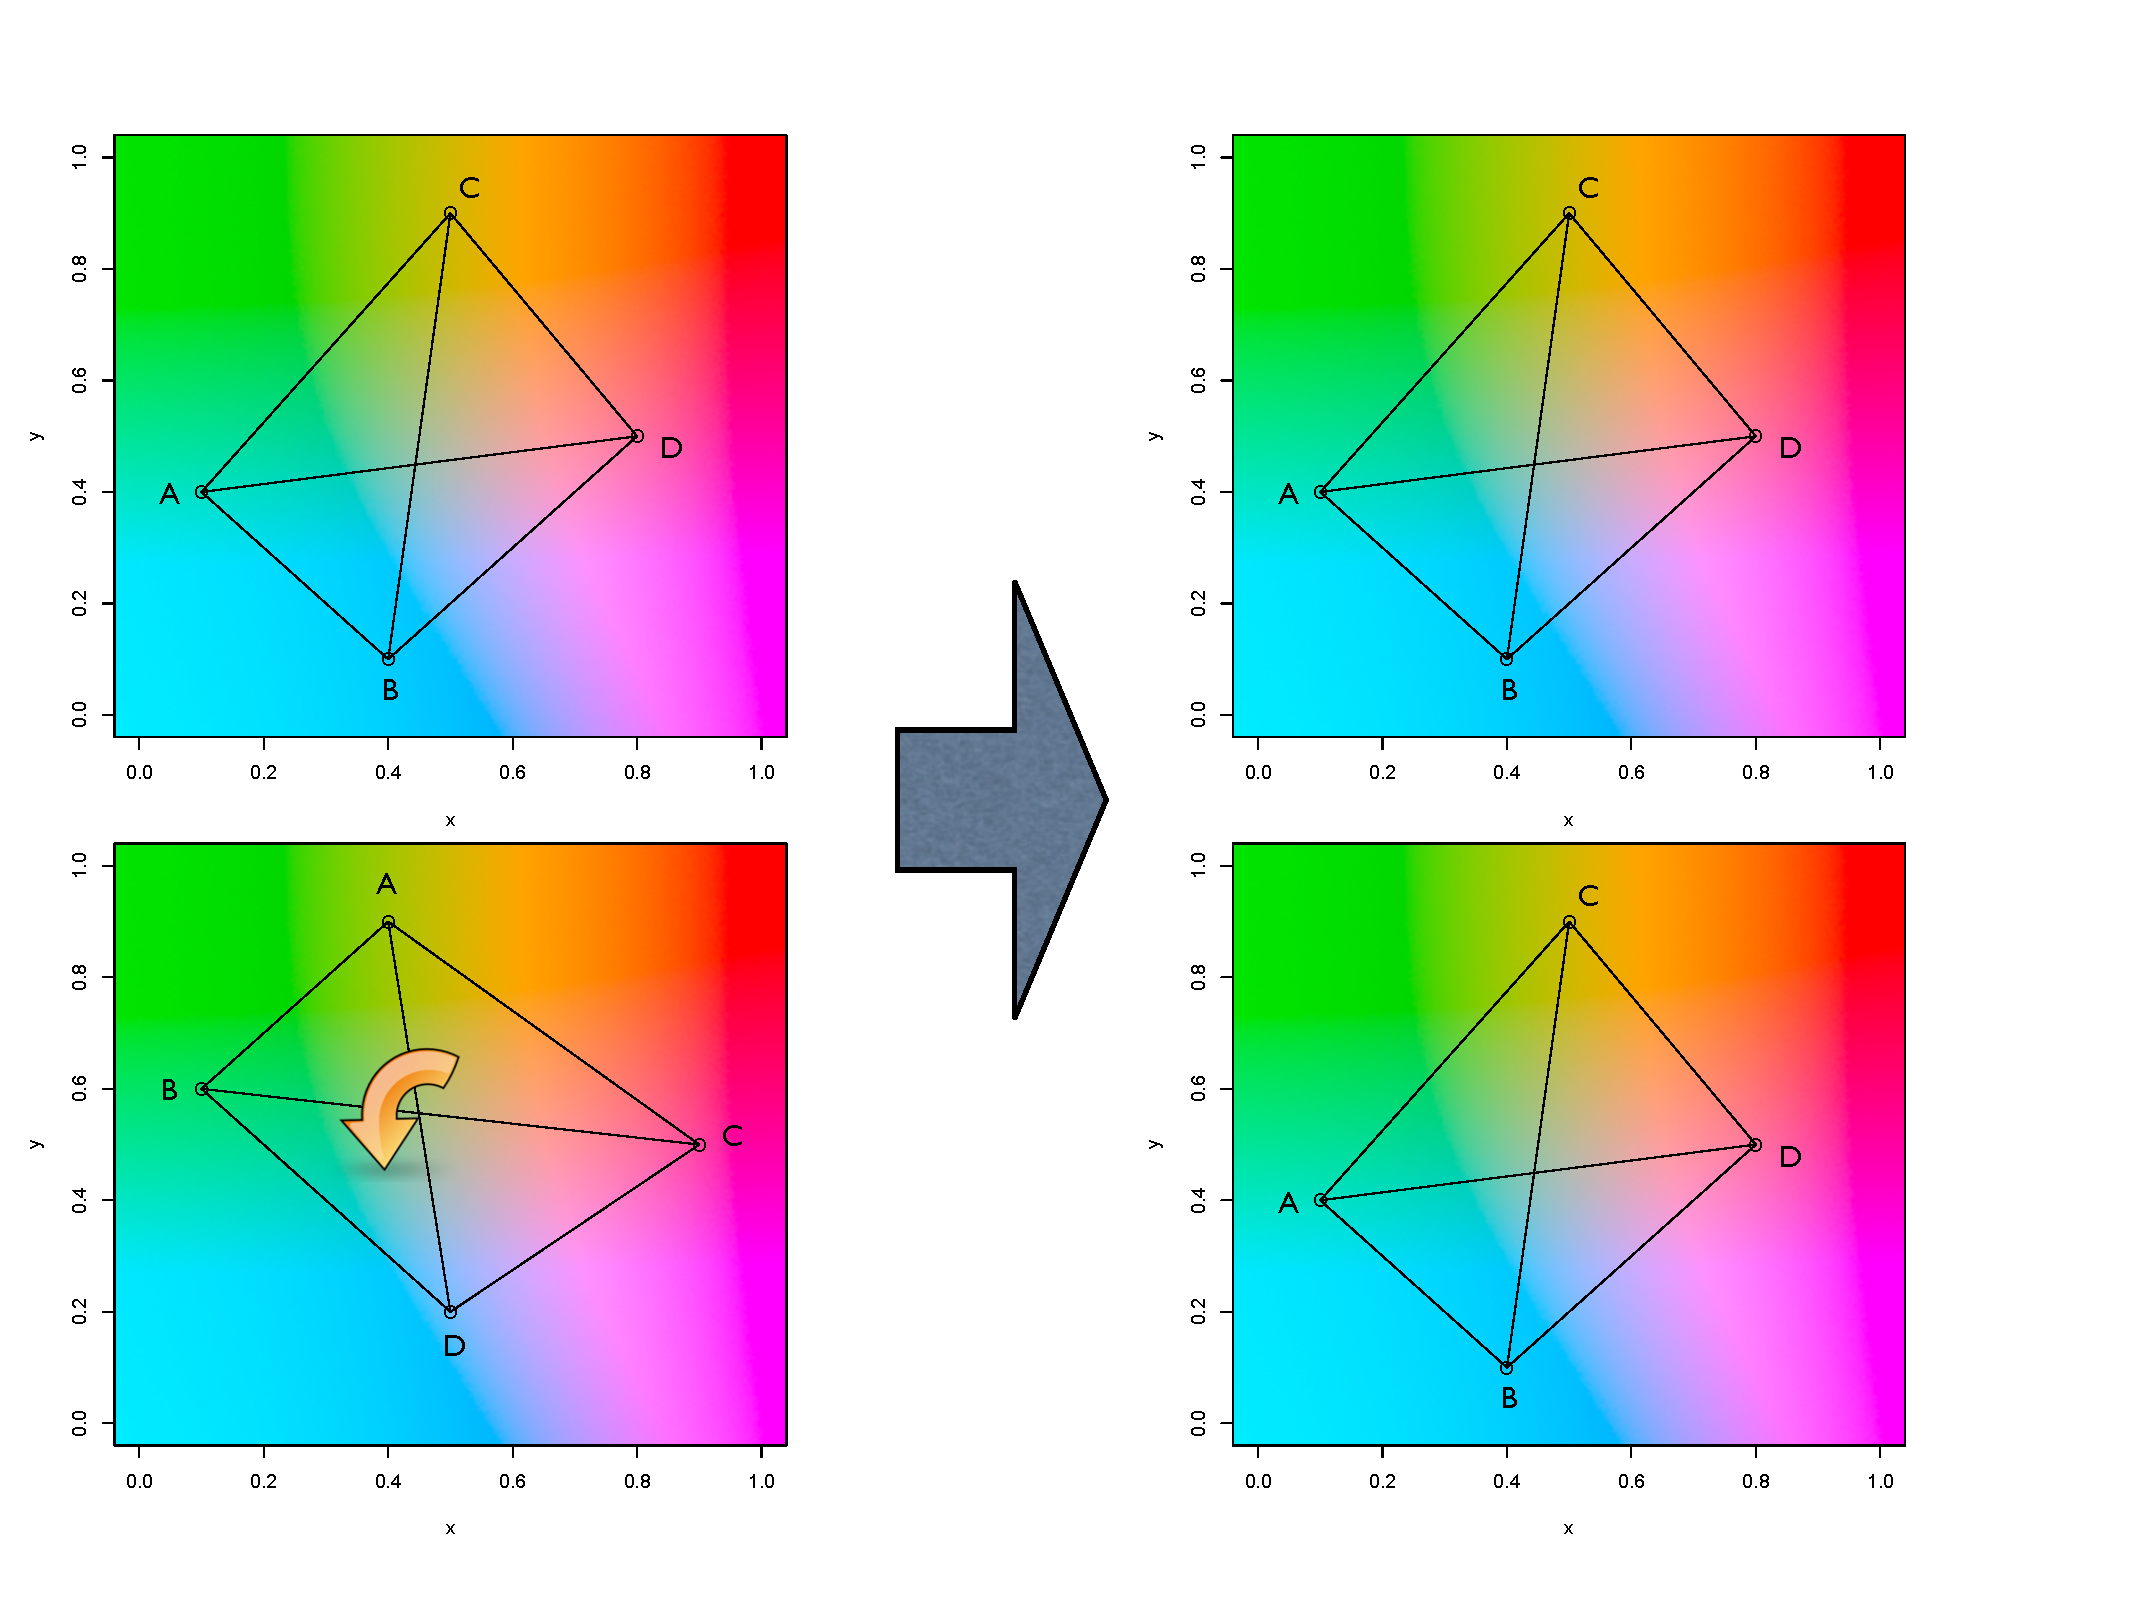
\includegraphics[width=\textwidth]{figures/chap2_rotate.pdf}}
\caption[Color Optimization by Rotation]{An example of color optimization by rotating.}\label{fig:chap2_rotate}
\end{figure}

A useful feature is, all the points in the color space can be arbitrarily rotated and/or flipped, without changing the distance between any pair of symbols within a column. For instance, all reds and all greens are virtually identical in the sense of distances and quality of alignment. Converting them into the same color pattern will better support this idea and remove unnecessary color noises.

\begin{figure}[hbt]
\center{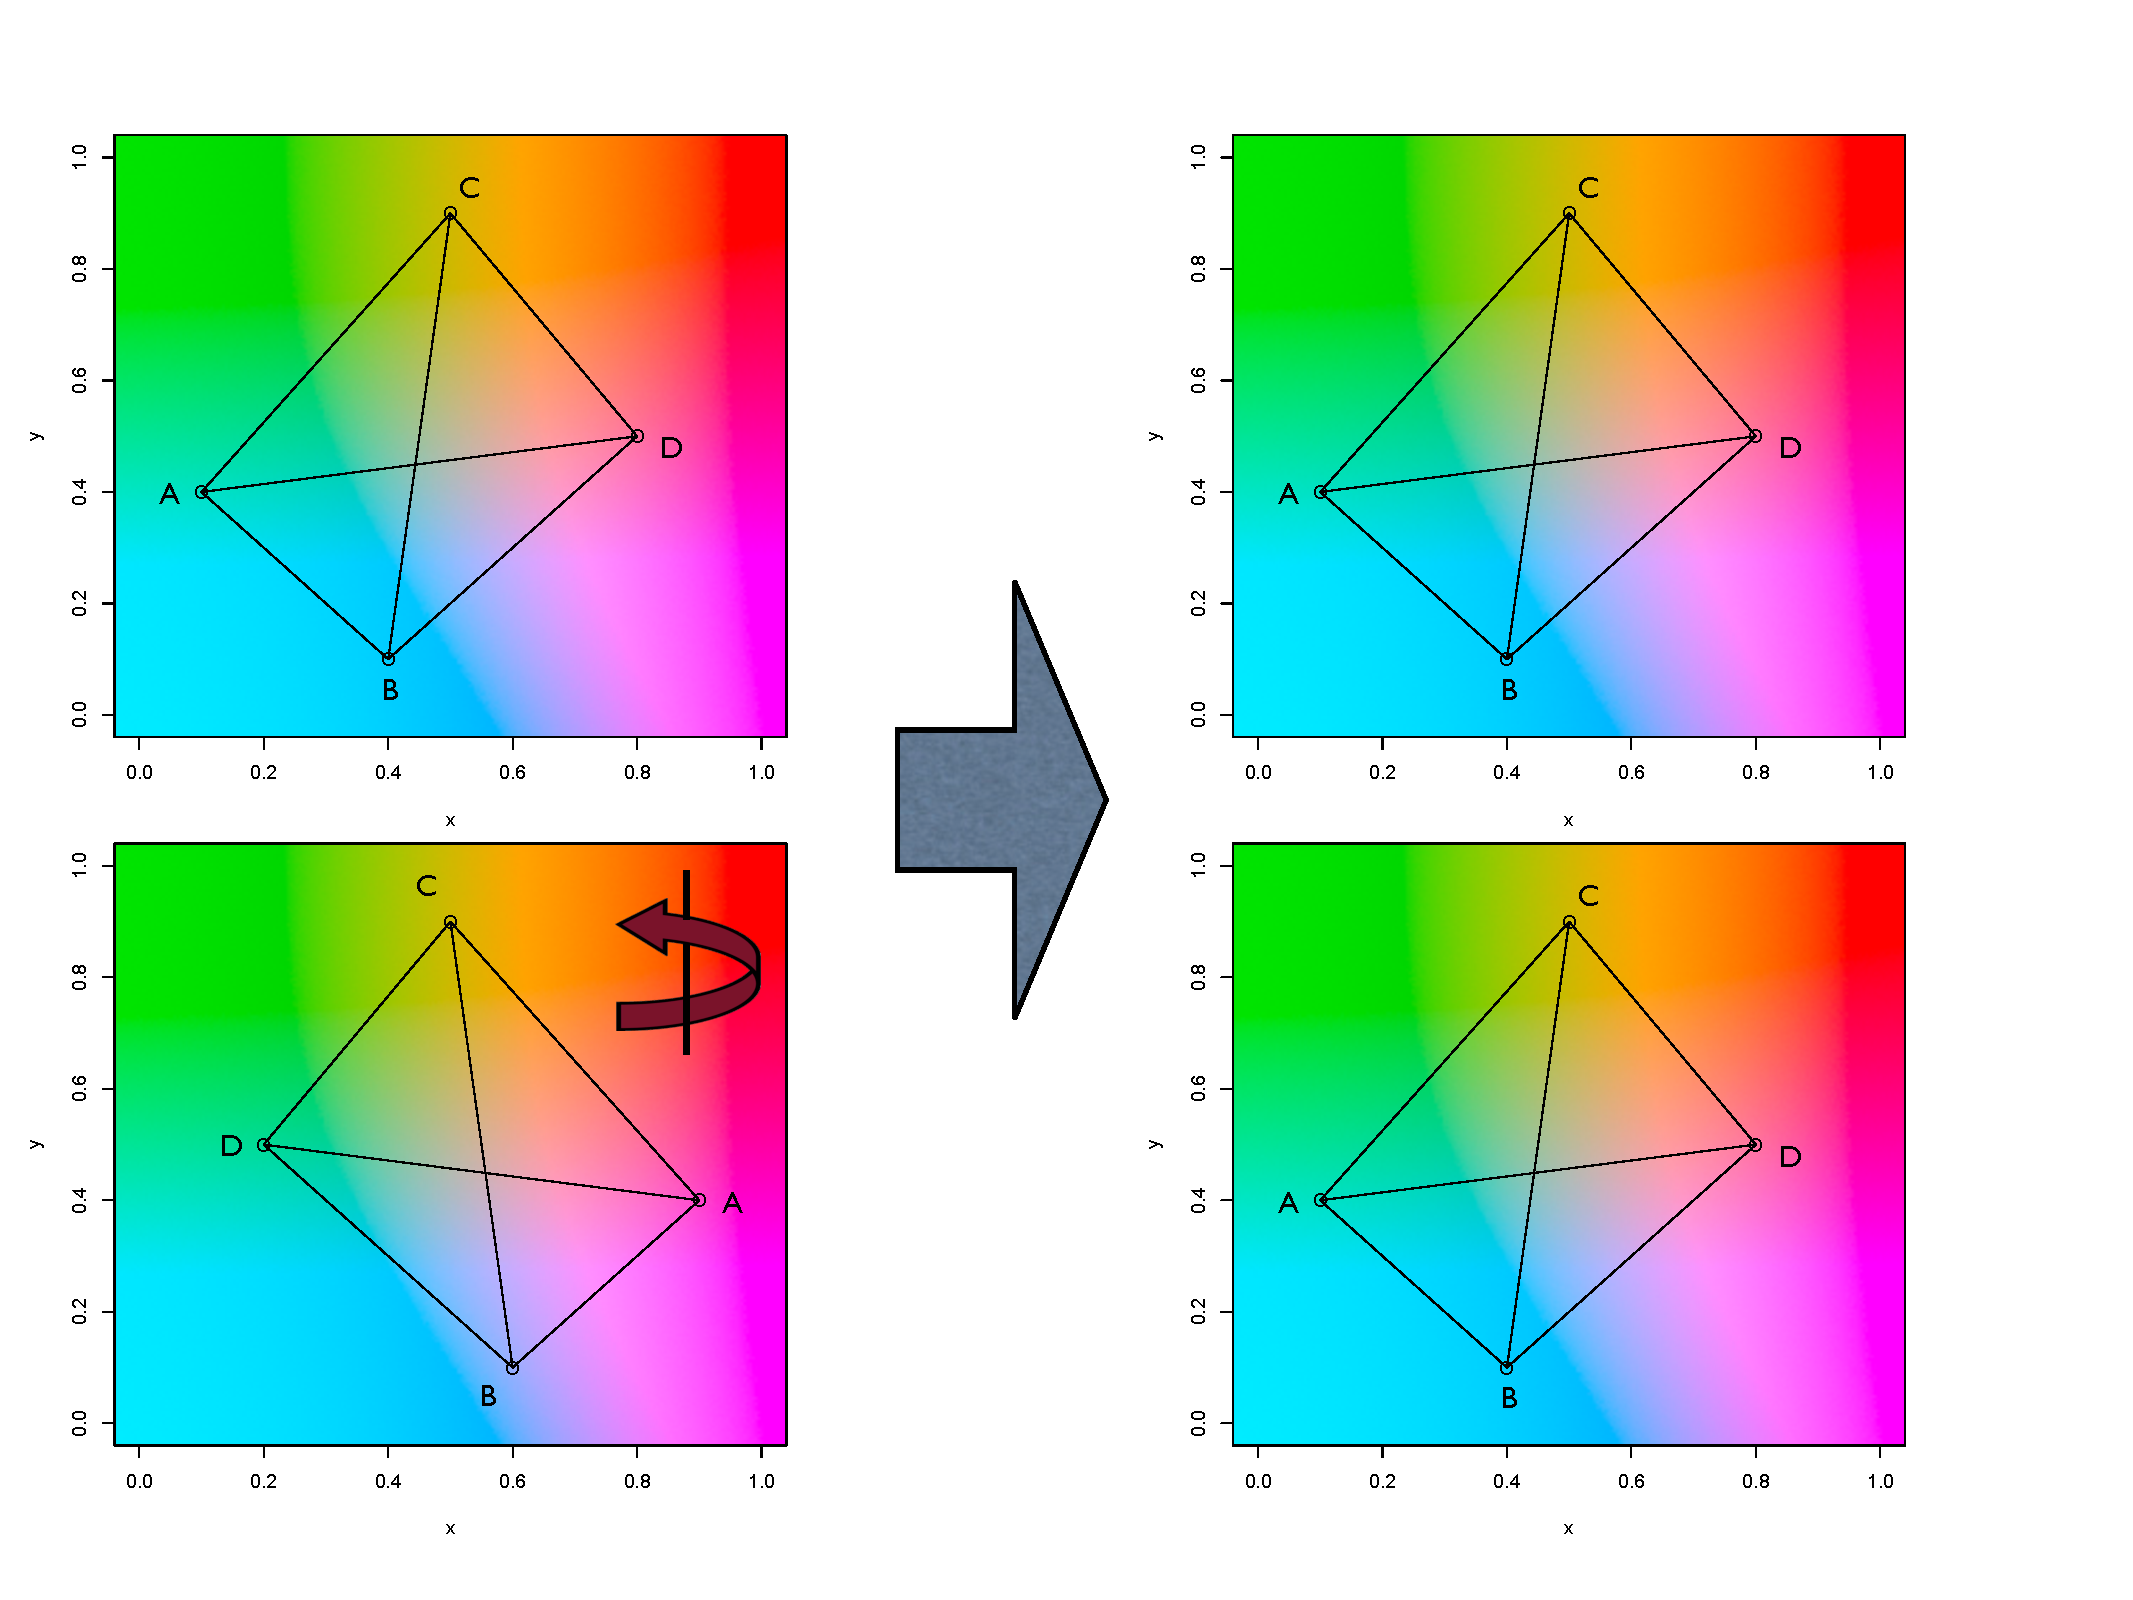
\includegraphics[width=\textwidth]{figures/chap2_flip.pdf}}
\caption[Color Optimization by Flipping]{An example of color optimization by flipping.}\label{fig:chap2_flip}
\end{figure}

To optimize our color assignment, we define a penalty function to quantify the overall noise level of an alignment. This function calculates the color variance within each row and sum them up. By rotating and flipping, the ideal color assignment should result in the lowest penalty value.

For larger MSAs, finding the exact optimum may become time-consuming and sometimes impractical. Sub-optimal results are also acceptable for visualization purpose. In Mavis, we use an approximate solution to speed up the optimization procedure.

\section{MSA Visualization}

Mavis creates a colored matrix for an MSA. Users may choose to display residue symbols or not. The user interface is available in a web browser, in order to achieve better flexibility and portability. Other user interfaces are also provided for devices like mobile phones and tablets.

\begin{figure}[hbt]
\center{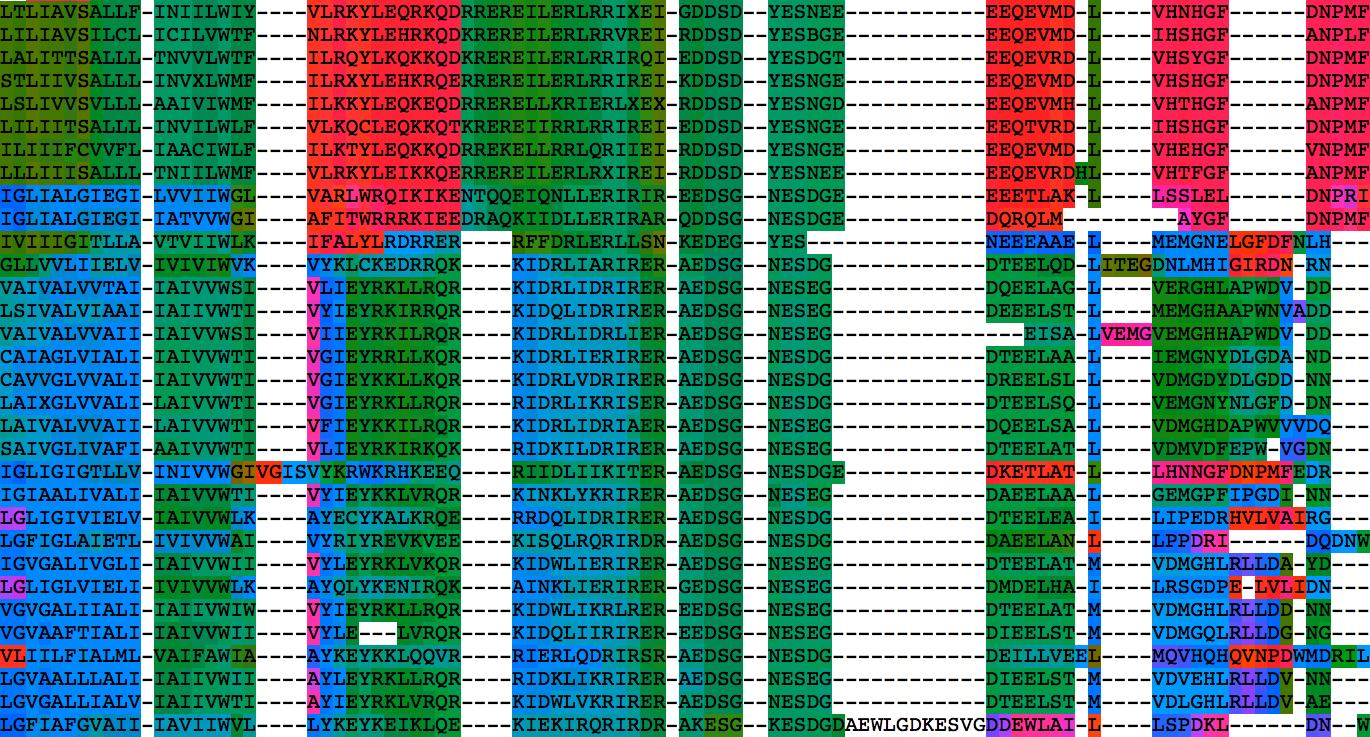
\includegraphics[width=0.72\textwidth]{figures/chap2_msa.png}}
\caption[Example of MSA Coloring Result]{An example of MSA coloring result.}\label{fig:chap2_msa}
\end{figure}

An API between the front-end and the back-end is designed to make the system extensible for more add-ons and user interfaces.

\chapter{Algorithms}\label{chap:Algorithms}

The algorithm of color computation consists of five stages. First, multidimensional scaling reduces the number of dimensions and convert the confidence/similarity scores into coordinates. Second, coordinates are mapped onto part of the \emph{CIE Lab color space} \cite {McLAREN:1976aa}, and colors are created. Third, colors are flipped and rotated to smooth the graph and remove color noises. Finally, calculate the average color/hue of each sequence, sort them, and output for further display.

\section{Multidimensional Scaling}

This stage begins with the confidence scores described above. Each column in the MSA has a complete set $C$ of pairwise scores. Each pair of non-gap symbols $i,j$ in this column has a score $c_{i,j}=c_{j,i} \in [0,1]$. Here 1 stands for absolute confidence or similarity, while 0 for the opposite.

This dataset can be easily converted to a set $D$ of dissimilarities or distances between two symbols, by $$d_{i,j}=d_{j,i}=1-c_{i,j}$$

These distance values are re-organized as an $n \times n$ symmetric distance matrix $M$
\[ \begin{array}{cccccc}
            & \mbox{1}  & \mbox{2}  & \mbox{3}  & \mbox{...}  & n       \\
\mbox{1}    & 0         & d_{1,2}   & d_{1,3}   & \cdots      & d_{1,n} \\
\mbox{2}    & d_{2,1}   & 0         & d_{2,3}   & \cdots      & d_{2,n} \\
\mbox{3}    & d_{3,1}   & d_{3,2}   & 0         & \cdots      & d_{3,n} \\
\cdots      & \cdots    & \cdots    & \cdots    & \cdots      & \cdots  \\
n           & d_{n,1}   & d_{n,2}   & d_{n,3}   & \cdots      & 0 \end{array} \]
where $n$ is the number of non-gap symbols in the current column.

These $n$ symbols are placed into a two-dimensional space, in which the distances between each other are still preserved as much as possible. This procedure involves a statistical technique called \emph{classical multidimensional scaling (classical MDS)}, also known as \emph(Torgerson-Gower scaling) or \emph{principle coordinates analysis (PCoA)} \cite{GOWER01121966}. Multidimensional scaling takes a distance matrix and assigns a coordinate to each item in a lower dimensional space, such that the Euclidean distance between any two coordinates is approximately equal to the original distance value between the corresponding items.

An statistical function called \emph{cmdscale()} \cite{R2009aa} is utilized in this multidimensional scaling procedure. This function is written in R, which is a programming language for statistical computing \cite{Gentleman:aa}, and is provided in R’s stat package. It reads a distance matrix and returns a set of points in a $k$-dimensional space, where $k$ is a user-defined parameter to the function, and must be less than the number of points $n$. \cite{Cailliez:1983aa,Cox:2008aa}

In our approach, $k$ is set to 2, meaning the distance matrix is scaled down to a two-dimensional space. However, a column of an MSA may have as few as one or two non-gap symbols, so that the distance matrix of this column is only $1 \times 1$ or $2 \times 2$. In such cases, $k=2$ will not be a valid parameter to \emph{cmdscale()} because of the $k<n$ requirement. So we let
\[
k = \left\{ \begin{array}{ll}
0 & \mbox{if $n=1$} \\
1 & \mbox{if $n=2$} \\
2 & \mbox{otherwise}
\end{array}
\right.
\]

Then we perform the multidimensional scaling on the distance matrix $M$. When $n<2$, the generated coordinates are lower than two-dimensional, and the missing coordinate values are filled by zeros.

\section{Color Space Mapping}

The above procedure returns a set $P$ of $n$ coordinates $(x,y)$ in a two-dimensional space, representing the $n$ symbols in a column of a multiple sequence alignment. This two-dimensional space is further mapped to a three-dimensional color space.

The CIE Lab color space \cite {McLAREN:1976aa} is a color-opponent space. The name \emph{Lab} stands for the three dimensions: $L$ for lightness, and $a$ and $b$ for the color opponents based on nonlinearly compressed \emph{CIE XYZ color space} coordinates \cite{CIE:1932aa,Smith:1931aa}. Compared to the \emph{RGB} and \emph{CMYK} color models, the design of Lab color emphasizes more on approximating human vision rather than physical devices. This feature makes it suitable for our visualization purpose. \cite{Margulis:2005aa}

Coordinates in $P$ have only two dimensions $x$ and $y$. To map $P$ to the three-dimensional CIE Lab space, $L$ for lightness is set to a fixed value 75, and two other dimensions $a$ and $b$ are assigned as $x$ and $y$ scaled from $[0,1]$ to $[0, 100]$. $$a=x*100$$ $$b=y*100$$

At the end of this step, $n$ CIE Lab colors $(L, a, b)$ are created.

\section{Hue Rotation and Optimization}

One of the limitations in many previous MSA visualization techniques is, they introduced unnecessary confusion by using a fixed color scheme. Even for exactly same aligned columns, colors may be totally different, which won't represent any biological dissimilarities. To minimize this effect, we convert the colors from CIE Lab space to \emph{CIE LCH space}, and perform rotations to eliminate noisy colors to the greatest extent possible. In this way, we smooth the color pattern and emphasize the real similarities and dissimilarities among sequences and blocks.

The \emph{CIE LCH color space}, also known as polar-Lab color space, is a cylindrical transformation of the CIE Lab space so that the a and b axles are converted to a polar coordinate system. The radial coordinate $C$ measures \emph{chroma} and the angular coordinate $H$ measures \emph{hue}. LCH space makes it easier to rotate colors, by changing their \emph{hue} value. The CIE LCH colors can be converted from CIE Lab colors using an R library called \emph{colorspace} \cite{Ihaka:2009aa,Zeileis:2009aa}.

Hue values are circular, meaning $0$ and $2\pi$ are identical. Given two angles $p$ and $q$, the difference between them is given by $$\mathrm{diff}(p,q) = (p - q + \pi) \bmod 2\pi - \pi$$ This calculation returns the difference in the interval $[-\pi, \pi)$, or in degrees $[-180^{\circ}, 180^{\circ})$. The absolute value of the difference $$|\mathrm{diff}(p,q)| = |(p - q + \pi) \bmod 2\pi - \pi|$$ returns in the interval $[0, \pi]$, or in degrees $[0^{\circ}, 180^{\circ}]$.

Given a set $A$ of angles $a_i$, the average angle $\overline{A}$ is $$\overline{A}=\arctan{\frac{\displaystyle\sum_{i=1}^n \sin{a_i}}{\displaystyle\sum_{i=1}^n \cos{a_i}}}$$ and the variance $\mathrm{Var}(A)$ is $$\mathrm{Var}(A)=\frac{\displaystyle\sum_{i=1}^n \mathrm{diff}(\overline{A}-a_i)^2}{n}$$

Given a colored MSA $Z$ with $m$ rows and $n$ columns, to estimate its overall noise level, a penalty function $\mathrm{pen}(Z)$ is defined by $$\mathrm{pen}(Z)=\displaystyle\sum_{j=1}^m \mathrm{Var}(h_{1j},h_{2j},\cdots,h_{nj})$$ where $h_{ij}$ is the hue value of the symbol at the $i$th column and $j$th row.

We look for an optimized set $R$ of $n$ rotation angles $r_i$, such that after rotating each hue in every $i$th column of $Z$ clockwise by $r_i$, the rotated MSA $Z^\prime$ achieves the minimized return value of the penalty function $\mathrm{pen}(Z^\prime)$.

The optimization procedure is performed by R's general-purpose optimization function \emph{optim()} \cite{R2009aa}. Among five available optimization algorithms provided by this function, we choose the \emph{bounded Broyden-Fletcher-Goldfarb-Shanno} (L-BFGS-B) method \cite{Byrd:1995aa}. This algorithm allows box constraints, meaning each variable can be given a lower and/or upper bound. Plus, it uses a limited amount of memory. The initial values are set to 0 and boundaries to $[0, 2\pi]$. More detailed comparison between different optimization functions and algorithms will be discussed later in Chapter 6.

\section{Hue Flipping}

One characteristic of the coordinates generated from multidimensional scaling is, they can not only be rotated, but also flipped, without changing the distances between each other. Adding flipping ability to the above rotation optimization procedure may result in lower minimal penalty values and better coloring results. To keep the penalty function simple and fast, we perform a heuristic flipping \emph{before} the rotation step.

For each pair of adjacent columns $C_i$ and $C_{i+1}$, $1 \le i \le n-1$, compare their hues row by row. Rows with gaps in these two columns are not take into consideration. For those rows with non-gap symbols on both sides, record their hue values $$h_{i,1},h_{i+1,1},h_{i,2},h_{i+1,2},\cdots,h_{i,k},h_{i+1,k}$$ into two lists $H_i$ and $H_{i+1}$: $$H_i=h_{i,1},h_{i,2},\cdots,h_{i,k}$$ $$H_{i+1}=h_{i+1,1},h_{i+1,2},\cdots,h_{i+1,k}$$

In both lists, compare two neighboring hue values $h_{i,j}$ and $h_{i,j+1}$, $1\le j\le k-1$, using diff$()$ function described in section 3.3. If diff$(h_{i,j},h_{i,j+1})<-\frac{\pi}{8}$, the change from $h_{i,j}$ to $h_{i,j+1}$ is called a \emph{clockwise change}; if diff$(h_{i,j},h_{i,j+1})>\frac{\pi}{8}$, the change is called a \emph{counterclockwise change}; otherwise, it's considered to be unchanged.

If a column contains more clockwise changes than counterclockwise changes, it's called \emph{clockwise column}; if it contains more counterclockwise changes, it's called \emph{counterclockwise column}; otherwise, it's a neutral column. Note that since gap rows are filtered out of the comparison, the type of a column may change when compared to different adjacent columns. For instance, a column may be clockwise compared to the previous column, and counterclockwise compared to the next column.

If two adjacent columns are in opposite types, flip the latter one to make them in same type. Then the flipped alignment are sent back to the procedure discussed in section 3.3.

\section{Sequence Sorting}

The alignment graph is supposed to provide information on how sequences will group with each other. We sort sequences after coloring optimization, based on the average hue of each one, which is calculated by the average angle function proposed previously in section 3.3.

The fact that hue values are circular, results in an additional question on where to cut the circle to get a sorted list of sequences. In a sorted circle of $n$ average hue values, $h_1,h_2,\cdots,h_n$, we calculate the absolute difference between each pair of adjacent ones ($h_1$ is adjacent to $h_n$). $$\Delta h_{1,2}=|\mathrm{diff}(h_1,h_2)|$$ $$\Delta h_{2,3}=|\mathrm{diff}(h_2,h_3)|$$ $$\cdots$$ $$\Delta h_{n,1}=|\mathrm{diff}(h_n,h_1)|$$ Then, the circle is split at the biggest gap $$\Delta h_{max}=\Delta h_{i,i+1}=|\mathrm{diff}(h_i,h_{i+1})|$$ to best avoid separating similar sequences.

\chapter{Implementation}\label{chap:Implementation}

We implemented the entire visualization pipeline on a Mac OS X server. The implementation consists of an R script as back-end, a Perl CGI script as API, and an HTML/JavaScript web page as user interface.

The R script \emph{coloring.r} takes the pair-wise similarity score file as input, performs multidimensional scaling and color optimization, sorts sequences, and output colors and sequence information into two tab-separated files \emph{colors.tsv} and \emph{seqinfo.tsv}. The front-end web page takes an alignment ID as parameter and sends it to the API. The Perl CGI script parses the color file and sequence information file, along with the FASTA-format alignment file, and sends them back to front-end in JSON format \cite{crockford2006application}. The front-end uses JavaScript to generate the alignment matrix and render it with colors and symbol letters.

\section{R Script}

The script \emph{coloring.r} begins with reading three arguments from command-line calls: score file name, colors file name and sequence information file name. The first file is for input and the latter two are for output. An example of calling this script on UNIX operating system is given below.
\begin{verbatim}
  Rscript coloring.r data/score.tsv data/colors.tsv data/seqinfo.tsv
\end{verbatim}

The file \emph{score.tsv} contains four columns separated by tabs: column number, first row number, second row number, and similarity score between these two rows in this column. The row and column numbers start from 1, and the similarity score values range from 0 to 1. Figure \ref{fig:score.tsv} shows a few example lines in a \emph{score.tsv} file.
\begin{figure}[hb]
\begin{quote}
\begin{verbatim}
  #COL_NUMBER   #ROW_NUMBER_1   #ROW_NUMBER_2   #RES_PAIR_HIT/NALT
  1             1               2               1.000000
  1             1               6               0.933333
  1             1               10              0.866667
  1             2               6               0.933333
  1             2               10              0.866667
  1             6               10              0.133333
  2             1               6               1.000000
  2             1               10              1.000000
  2             6               10              1.000000
\end{verbatim}
\end{quote}
\caption[Example of Similarity Score File]{An example of similarity score file \emph{score.tsv}, showing the format of the file. The four columns are: column number, the first row number, the second row number, score value.}\label{fig:score.tsv}
\end{figure}

The script \emph{coloring.r} consists of four parts. The first part reads the input file, performs multidimensional scaling and create color for each symbol in the CIE LCH space. The second part rotates and flips color hues and optimize the penalty function. The third part sorts the sequences by their average hues and calculates each sequence’s average RGB color. The last part outputs the symbol colors and sequence information into corresponding files.

The color file \emph{colors.tsv} has five columns separated by tabs: column number, row number, and the symbol color in RGB triplet (red, green, blue) in the range from 0 to 1, which will be converted into hexadecimal format used in the user interface module. The sequence information file seqinfo.tsv also has five columns: row number, average hue from 0 to 360 degrees, and average color in RGB triplet. Figure \ref{fig:color.tsv} shows how a typical \emph{color.tsv} file looks like.
\begin{figure}[hb]
\begin{quote}
\begin{verbatim}
1       1       0.1065524      0.5616907       0.3943046
1       2       0.106256       0.5616652       0.3936842
1       6       0.1065487      0.5616904       0.3942968
1       10      0.1065581      0.5616912       0.3943165
2       1       0.09057406     0.5677889       0.2867890
2       2       0.09057406     0.5677889       0.2867890
2       6       0.09057406     0.5677889       0.2867890
2       10      0.09057406     0.5677889       0.2867890
3       1       0.07634505     0.5664451       0.2581746
3       6       0.1113592      0.570106        0.3250781
3       10      0.07634505     0.5664451       0.2581746
\end{verbatim}
\end{quote}
\caption[Example of Coloring Result File]{An example of coloring result file \emph{color.tsv}, showing the format of the file. The five columns are (from left to right): row number, average hue, red, green and blue.}\label{fig:color.tsv}
\end{figure}

\section{API}

A Perl CGI script \emph{api.pl} and a Perl package \emph{Mavis::API} act as the API between the R back-end and HTML/JavaScript front-end. The Perl CGI \emph{api.pl} takes two parameters from HTTP requests, \emph{action} and \emph{id}. The default action is \emph{alignment}, meaning the alignment information, including sequences, colors, average colors and order of sequences, should be returned. In this action, an additional \emph{id} parameter is expected as the alignment ID. Another available action is \emph{list}, which requests a list of all existing alignment IDs.

The API returns the query result to the web page in JSON (JavaScript Object Notation) format, which is a lightweight text-based data-interchange standard. JSON is derived from a subset of JavaScript syntax and can be easily parsed in JavaScript as well as many other languages, like Perl. We included the Perl JSON 2.51 module to provide JSON encoding/decoding ability to our API \cite{crockford2006application}.

Figure \ref{fig:api-res} is an example of the API response in JSON format:
\begin{figure}[hb]
\begin{quote}
\begin{verbatim}
  { "status"    : 1,
    "id"        : "demo",
    "colors"    : [ ["#666","#666","#666","#666"],
                    ["#665","#667","#667","#665"]],
    "sequences" : [ {"name":"Seq02", "color":"#26e", "seq":"DEMO"},
                    {"name":"Seq01", "color":"#26e", "seq":"DEMO"}]
  }
\end{verbatim}
\end{quote}
\caption[Example of API Response in JSON Format]{An example of Mavis API response in JSON format.}\label{fig:api-res}
\end{figure}

\section{User Interfaces}

We implement an web interface with HTML and JavaScript to send API requests and draw visualization graphs. The JavaScript code dynamically communicates with API, creates an HTML table, and fills in colors and symbols. This part is simplified by jQuery, which is a popular cross-platform JavaScript library that abstracts complicated DOM selection, CSS manipulation and Ajax effects.

\section{Design Principles}
\chapter{Results}\label{chap:Results}

To evaluate the validity and performance of our approach, we tested it in two different ways. First, we run it on a few artificial datasets, to see if it creates the color patterns as we expected. Then, we run it on the BAliBASE dataset, observe how alignment size, in both number of rows and columns, will affect the excution time, and compare it with other tools.

\section{Validity Test}

\emph{(Under construction)}

\section{Performance Test}

\emph{(Under construction)}

\chapter{Discussion}\label{chap:Discussion}

In this report, we introduced a new way of coloring and visualizing multiple sequence alignments based on symbol-symbol similarity scores. Our main objective has been to create an intuitive way of showing the quality and internal structure of an alignment, using colors, which is the most natural and sensible way for human eyes. The basic idea is, the greater the dissimilarity between sequences, the more obvious difference in colors.

Most previous techniques were based on fixed color schemes, meaning each sequence symbol, like an amino acid or a nucleotide, is assigned to a pre-selected color. This is of course a simple and straightforward solution, and is easy for observers to find a particular symbol or pattern. However, this fixed-scheme approach does not emphasize the relationship between adjacent columns and the internal regions and structures in the level of the whole alignment. This is the main reason why we don’t use any predetermined color scheme, but calculate colors only based on the distance matrices, and rotate and flip colors to make them as smooth as possible. This strategy brings significant improvement to the alignment coloring, by showing the conserved regions and blocks in same or similar colors, while those irrelevant ones in quite different colors.

Since we are to convert the scaled coordinates to colors, choosing a suitable color space is an fundamental task. At first we scaled the distance matrix down to a three-dimensional space and mapped it directly to the RGB color space. However, we soon found a problem, that some colors, like very dark ones and very light ones, did not perfectly serve the purpose of representing distances, yet made the graph more noisy. We realized that we don’t really need the whole color space and all possible colors. Instead, those colors with proper range of lightness and different hues will be enough to do the job. So we chose to scale down to a two-dimensional space and map it to CIE Lab space with a fixed lightness value (75). The reason why we didn’t choose one-dimensional scaling is that, a linear space either could not map to enough number of colors (for example, use only one primary color, like red), or could not preserve the distance information (for example, use only hues). So two dimensions is a good balance.

In R, there are several general purpose optimization packages which offer facilities for solving our color rotation and flipping problems. Two popular functions are optim() and nlminb() from package stats. Function optim() provides implementations of five algorithms: Broyden-Fletcher-Goldfarb-Shanno (BFGS), bounded BFGS (L-BFGS-B), conjugate gradient (CG), Nelder and Mead (Nelder-Mead), and simulated annealing (SANN). Nelder-Mead (Nelder and Mead 1965), which is the default one, returns robust results but is relatively slow. CG (Fletcher and Reeves 1964) in faster in larger optimization problems, but more fragile. BFGS is a balance, and L-BFGS-B further provides the ability of box constraints, that each variable can be given a lower/upper bound. SANN (Belisle 1992) is more powerful on rough surfaces but relatively slow. Another function nlminb() offers similar box constraint optimization and similar performance to L-BFGS-B, so these two algorithms are chosen to a further test.

Optimization algorithms always suffer from the local versus global minimum problem, and the final result are more or less unstable and depending on the initial values. To decide which one of L-BFGS-B and nlminb() is more stable in our approach, we run a test on both of them. The test dataset is the alignment of 44 Vpu protein sequences from Guidance. We randomly created 100 sets of initial values, performed optimizations, and see how the return value of the penalty function described in section 3.3 changed.
Algorithm	Minimum penalty	Aerage penalty	Maximum penalty	Standard deviation
Initial	
370,584
425,728
444,771
13,998
L-BFGS-B	
136,909
178,850
247,218
17,871
L-BFGS-B - run 3 times	
136,909
178,850
247,218
17,871
mlninb()	
146,759
181,688
426,535
34,579
mlninb() - run 3 times	
142,888
171,380
325,469
21,402


Obviously using L-BFGS-B is more stable than nlminb() on our test dataset.


%\section{Summary of Contributions}
%
%\subsection{Image Segmentation}
%
%\subsection{Cardiac Morphology and Function}
%
%\subsection{Coronary Artery Shape-Motion Analysis}
%
%%%%%%%%%%%%%%%%%%%%%%%%%%%%%%%%%%%%%%%%%%%%%%%%%%%%%%%%%%%%%%%%
%\section{Progression and Scope for Future Work}
%
%
%\subsection{Algorithm for the Automatic LV Blood Pool Segmentation
%from Short-Axis Dual-Contrast MR Data}
%
%%%%%%%%%%%%%%%%%%%%%%%%%%%%%%%%%%%%%%%%%%%%%%%%%%%%%%%%%%%%%%%%
%\subsection{Algorithm for the Automatic Delineation of Myocardial
%Contours in Short-Axis Cardiac Cine-bFFE MR Sequences}
%
%
%%%%%%%%%%%%%%%%%%%%%%%%%%%%%%%%%%%%%%%%%%%%%%%%%%%%%%%%%%%%%%%%
%\subsection{Algorithm for the Automatic Computation of EF from the Short-Axis Cardiac Cine-bFFE MR Sequences}
%
%
%%%%%%%%%%%%%%%%%%%%%%%%%%%%%%%%%%%%%%%%%%%%%%%%%%%%%%%%%%%%%%%%
%\subsection{Computational Framework for the 4D
%Shape-Motion Analysis of the LAD}
%
%
%%%%%%%%%%%%%%%%%%%%%%%%%%%%%%%%%%%%%%%%%%%%%%%%%%%%%%%%%%%%%%%%
%\subsection{Future Work}
%
%%%%%%%%%%%%%%%%%%%%%%%%%%%%%%%%%%%%%%%%%%%%%%%%%%%%%%%%%%%%%%%%

\chapter{Conclusion}\label{chap:Conclusion}

In this report, we introduced Mavis, a new way of coloring and visualizing multiple sequence alignments. Our main objective has been to create an intuitive way of showing the quality and internal structure of an alignment. We use colors, which is the most natural and sensible way for human eyes, to accomplish this goal. The basic idea is, the greater the dissimilarity between sequences, the more obvious difference in colors.

Most previous techniques were based on fixed color schemes, meaning each sequence symbol, like an amino acid or a nucleotide, is designated to a pre-selected color. This is of course a simple and straightforward solution, and is easy for observers to find a particular type or pattern of symbols. However, this fixed-scheme approach does not emphasize the relationship between adjacent columns and the internal regions and structures in the level of the whole alignment. This is the main reason why we do not use any predetermined color schemes.

In order to dynamically generate colors for an MSA, we require a user-input data set of symbol-symbol similarity (or alignment confidence) scores. This data set is converted into a set of distance matrices, one for each alignment column. Each distance matrix is then scaled to a two-dimensional space and mapped onto a CIE Lab color space to get colors. To optimize the result, the color space is rotated and flipped to reduce the overall color noise level as low as possible. This strategy brings significant improvement to the alignment coloring, by showing the well aligned regions in solid colors, while poorly aligned ones in various different colors.

Mavis is implemented in R, Perl, HTML, and JavaScript. The core algorithm written in R performs all the calculations. Perl CGI is used to set up an API between back-end and front-end. The API is designed in an extensible way and supports different user interfaces, even user-created ones. We provide a graphical user interface in HTML and JavaScript, which can be easily accessed over the Internet with any major web browsers.

We hope Mavis becomes a fast, light-weight, and easy-to-use tool for biologists who study comparative sequence data, and assists researchers to better analyze multiple sequence alignments, especially from functional, structural, and evolutionary perspectives.

\bibliographystyle{ieeetr}
\bibliography{references}

\appendix
\renewcommand{\appendixname}{Appendix}

\lstset{
basicstyle=\footnotesize\ttfamily,
numbers=left,
numberstyle=\tiny,
stepnumber=2,
numbersep=25pt,
tabsize=2,
extendedchars=true,
breaklines=true,
}

\begin{appendices}

\chapter{Color-generating Script}
\section*{\emph{coloring.R}}
\lstinputlisting{source/coloring.R}

\chapter{API Script}
\section*{\emph{api.pl}}
\lstinputlisting{source/api.pl}
\section*{\emph{Mavis/API.pm}}
\lstinputlisting{source/API.pm}

\chapter{User Interface Script}
\section*{\emph{mavis.js}}
\lstinputlisting{source/mavis.js}

\end{appendices}

\end{document}
